	\subsection{Pemahaman Teori}
		\begin{enumerate}
			\item	\begin{itemize}
						\item Fungsi adalah bagian dari program yang berupa blok kode yang diberikan nama dan nama tersebut berguna untuk memanggil fungsi tersebut.
					
						\item Inputan fungsi adalah sebuah fungsi yang telah di sediakan pada library python, yang berguna untuk menerima inputan dari user.
					
						\item Kembalian fungsi adalah sebuah nilai balikan yang diberikan oleh sebuah fungsi yang dibuat.
					\end{itemize}
					
					Contoh Program : 
					\lstinputlisting[language=Python, firstline=2, lastline=8]{src/chapter3/teori_1174043_chap3.py}
					
			\item paket adalah sebuah cara yang dilakukan untuk memanggil file script python, yang nantinya akan digunakan fungsi fungsi yang terdapat pada file script yang dipanggil tersebut. cara pemanggilan paket dengan cara :
				\begin{verbatim}
				import scriptFilePython
				\end{verbatim}
			
			Contoh Program :
			\lstinputlisting[language=Python, firstline=11, lastline=11]{src/chapter3/teori_1174043_chap3.py}
			
			\item	\begin{itemize}
						\item Kelas merupakan sebuah cetakan atau Blueprint yang berguna untuk mencetak objek.
						
						\item Objek merupakan sebuah objek yang dari proses hasil dari cetakan atau blueprint.
						
						\item Atribut merupakan penggambaran data yang bisa memberikan sebuah informasi kelas atau objek dimana atribut tersebut berada.
						
						\item Method merupakan fungsi atau prosedur yang bergabung dengan sebuah objek dan juga atribut.
					\end{itemize}
					
					Contoh Program :
					\lstinputlisting[language=Python, firstline=14, lastline=17]{src/chapter3/teori_1174043_chap3.py}
					
			\item cara pemanggilan library kelas dari instansiasi, adalah dengan cara mengubah library kelas yang dipanggil menjadi sebuah objek.
			
			Contoh Program : 
			\lstinputlisting[language=Python, firstline=22, lastline=24]{src/chapter3/teori_1174043_chap3.py}
			
			\item Jadi pemakaian paket dengan perintah from kalkulator import penambahan berguna untuk menghemat memori pemakaian pada program, karena hanya memanggil fungsi yang diperlukan saja pada library yang terpanggil. cara memanggilnya dengan cara :
				\begin{verbatim}
				from scripFilePython import namaFungsi, namaFungsi2
				\end{verbatim}
				
			Contoh Program :
			\lstinputlisting[language=Python, firstline=27, lastline=27]{src/chapter3/teori_1174043_chap3.py}
			
			\item \lstinputlisting[language=Python, firstline=30, lastline=35]{src/chapter3/teori_1174043_chap3.py}
			
			\item \lstinputlisting[language=Python, firstline=38, lastline=42]{src/chapter3/teori_1174043_chap3.py}
			
		\end{enumerate}
		
	\subsection{Keterampilan Pemrograman}
		\begin{enumerate}
			\item Jawaban soal no 1
				\lstinputlisting{src/chapter3/chap3_1174043_no1.py}
				
				\subitem Pada gambar \ref{gambar1} merupakan hasil compile kode programmnhya

				\begin{figure} [ht]
					\centerline{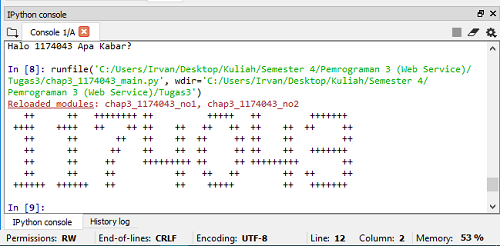
\includegraphics[width=0.6\textwidth]{figures/chapter3/1_1174043.png}}
					\caption{Jawaban No. 1}
					\label{gambar1}
				\end{figure}

				
				
			\item Jawaban soal no 2
				\lstinputlisting{src/chapter3/chap3_1174043_no2.py}

				\subitem Pada gambar \ref{gambar2} merupakan hasil compile kode programmnhya

				\begin{figure} [ht]
					\centerline{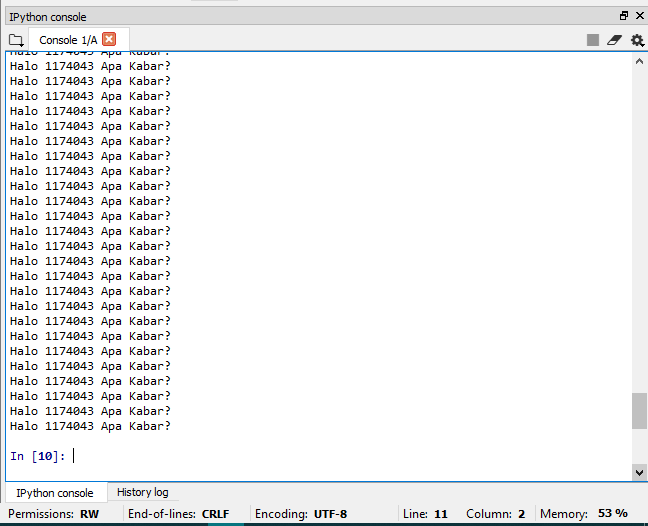
\includegraphics[width=1\textwidth]{figures/chapter3/2_1174043.png}}
					\caption{Jawaban No. 2}
					\label{gambar2}
				\end{figure}

			
			
			\item Jawaban soal no 3
				\lstinputlisting{src/chapter3/chap3_1174043_no3.py}

				\subitem Pada gambar \ref{gambar3} merupakan hasil compile kode programmnhya				

				\begin{figure} [ht]
					\centerline{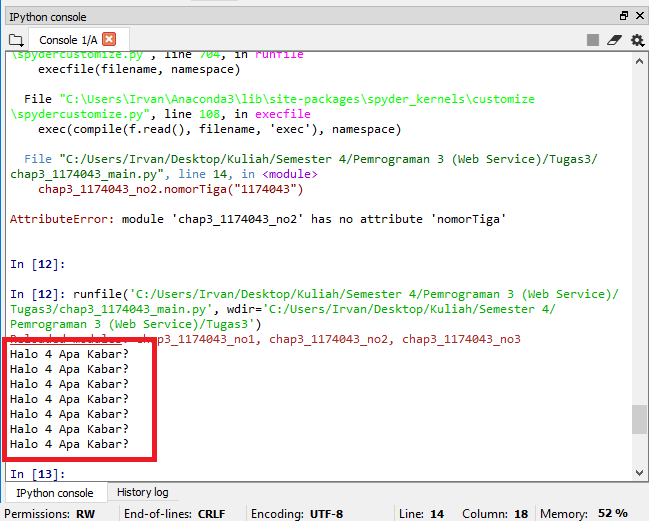
\includegraphics[width=1\textwidth]{figures/chapter3/3_1174043.png}}
					\caption{Jawaban No. 3}
					\label{gambar3}
				\end{figure}

			
				
			\item Jawaban soal no 4
				\lstinputlisting{src/chapter3/chap3_1174043_no4.py}

				\subitem Pada gambar \ref{gambar4} merupakan hasil compile kode programmnhya								

				\begin{figure} [ht]
					\centerline{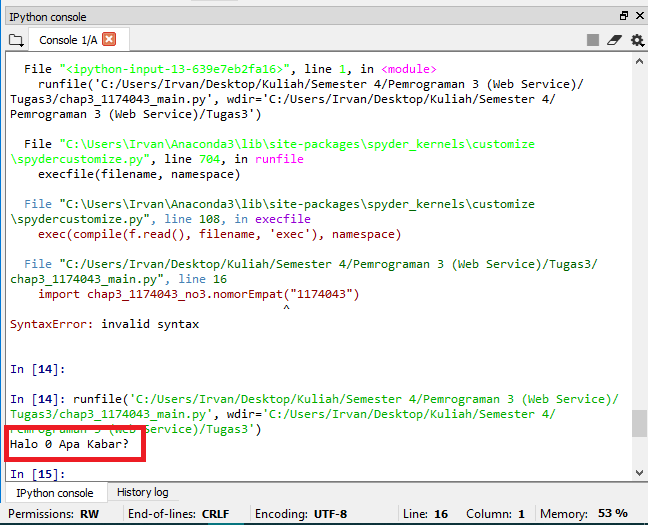
\includegraphics[width=1\textwidth]{figures/chapter3/4_1174043.png}}
					\caption{Jawaban No. 4}
					\label{gambar4}
				\end{figure}

				
			\item Jawaban soal no 5
				\lstinputlisting{src/chapter3/chap3_1174043_no5.py}

				\subitem Pada gambar \ref{gambar5} merupakan hasil compile kode programmnhya				

				\begin{figure} [ht]
					\centerline{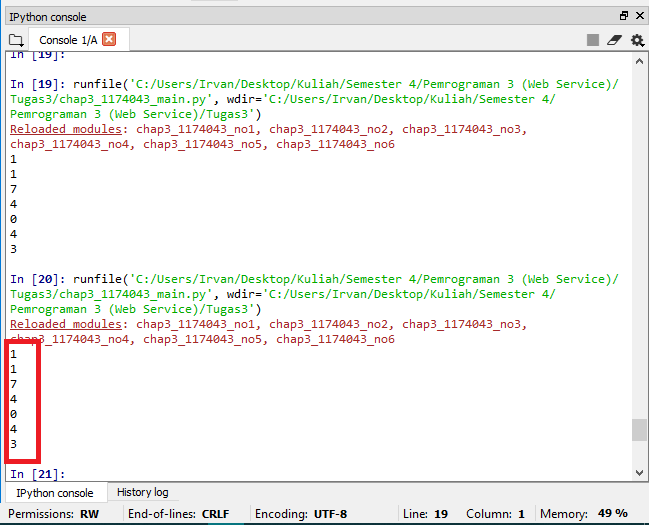
\includegraphics[width=1\textwidth]{figures/chapter3/5_1174043.png}}
					\caption{Jawaban No. 5}
					\label{gambar5}
				\end{figure}

				
			\item Jawaban soal no 6
				\lstinputlisting{src/chapter3/chap3_1174043_no6.py}
				
				\subitem Pada gambar \ref{gambar6} merupakan hasil compile kode programmnhya	

				\begin{figure} [ht]
					\centerline{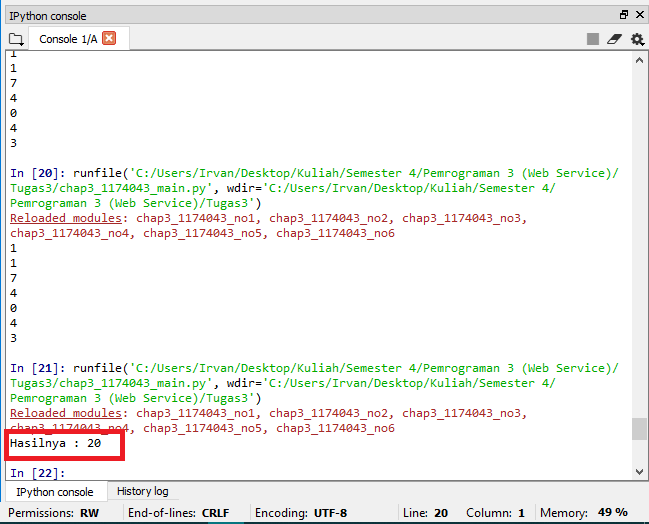
\includegraphics[width=1\textwidth]{figures/chapter3/6_1174043.png}}
					\caption{Jawaban No. 6}
					\label{gambar6}
				\end{figure}

				
			\item Jawaban soal no 7
				\lstinputlisting{src/chapter3/chap3_1174043_no7.py}

				\subitem Pada gambar \ref{gambar7} merupakan hasil compile kode programmnhya					

				\begin{figure} [ht]
					\centerline{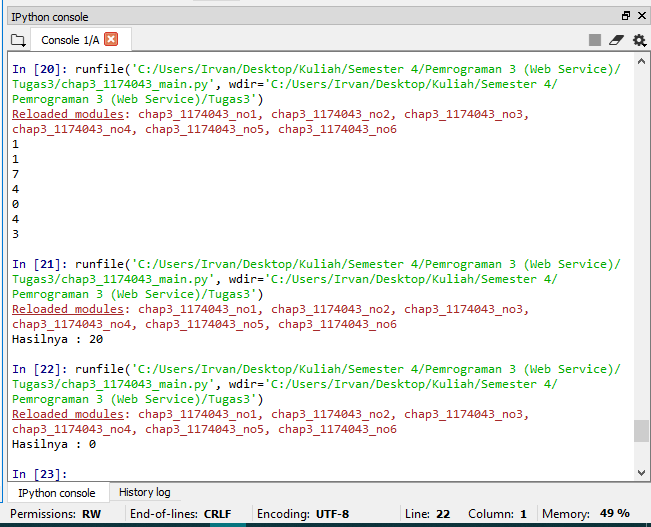
\includegraphics[width=1\textwidth]{figures/chapter3/7_1174043.png}}
					\caption{Jawaban No. 7}
					\label{gambar7}
				\end{figure}

				
			\item Jawaban soal no 8
				\lstinputlisting{src/chapter3/chap3_1174043_no8.py}

				\subitem Pada gambar \ref{gambar8} merupakan hasil compile kode programmnhya					

				\begin{figure} [ht]
					\centerline{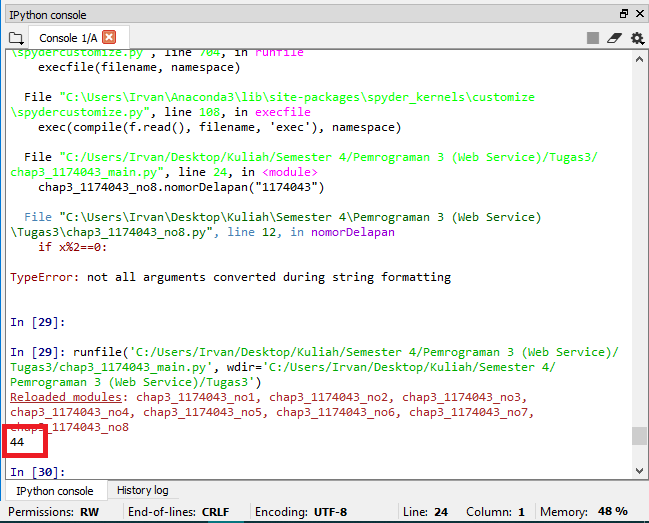
\includegraphics[width=1\textwidth]{figures/chapter3/8_1174043.png}}
					\caption{Jawaban No. 8}
					\label{gambar8}
				\end{figure}

			
				
			\item Jawaban soal no 9
				\lstinputlisting{src/chapter3/chap3_1174043_no9.py}
				
				\subitem Pada gambar \ref{gambar9} merupakan hasil compile kode programmnhya

				\begin{figure} [ht]
					\centerline{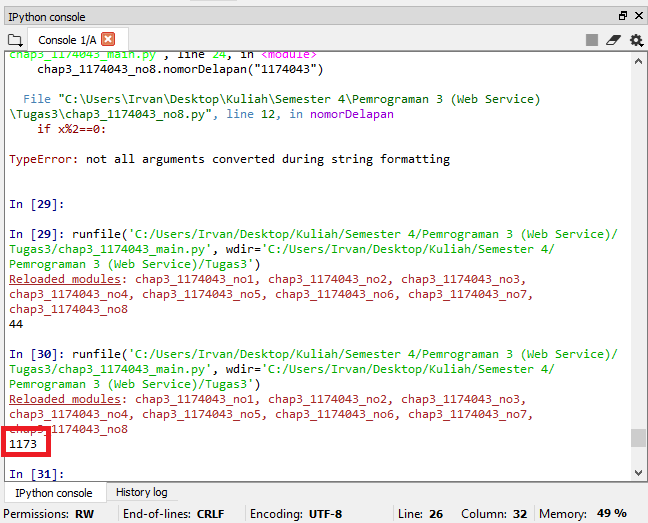
\includegraphics[width=1\textwidth]{figures/chapter3/9_1174043.png}}
					\caption{Jawaban No. 9}
					\label{gambar9}
				\end{figure}

				
			\item Jawaban soal no 10
				\lstinputlisting{src/chapter3/chap3_1174043_no10.py}
				
				\subitem Pada gambar \ref{gambar10} merupakan hasil compile kode programmnhya

				\begin{figure} [ht]
					\centerline{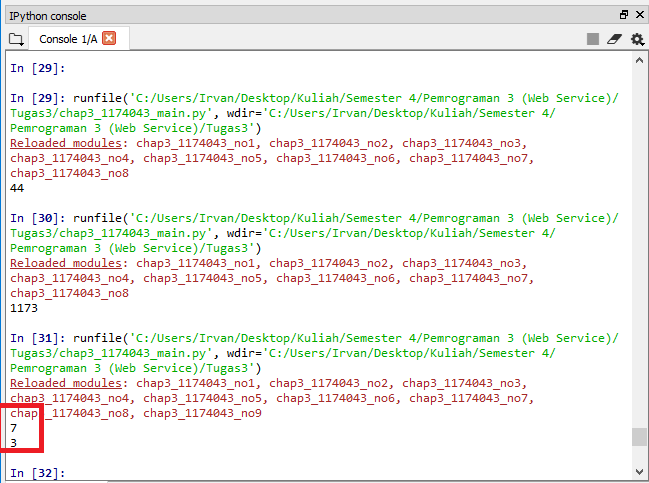
\includegraphics[width=1\textwidth]{figures/chapter3/10_1174043.png}}
					\caption{Jawaban No. 10}
					\label{gambar10}
				\end{figure}

				
			\item Jawaban soal no 11
			
				File 3lib.py
				\lstinputlisting{src/chapter3/chap3_1174043_3lib.py}
				
				File main.py
				\lstinputlisting{src/chapter3/chap3_1174043_main.py}
				
				\subitem Pada gambar \ref{gambar11} merupakan hasil compile kode programmnhya

				\begin{figure} [ht]
					\centerline{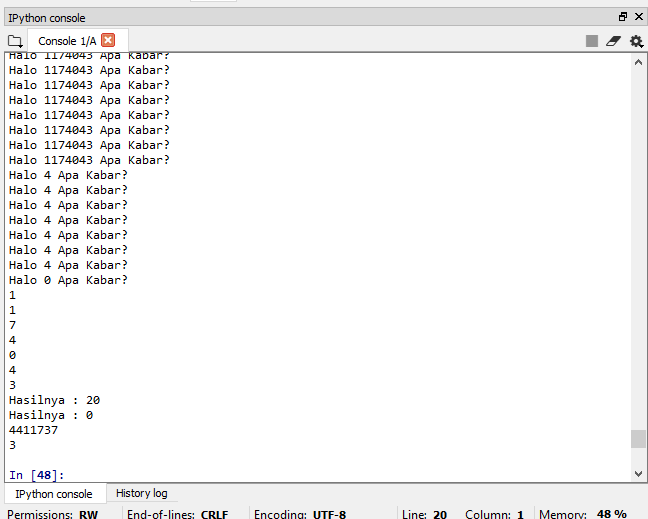
\includegraphics[width=1\textwidth]{figures/chapter3/11_1174043.png}}
					\caption{Jawaban No. 11}
					\label{gambar11}
				\end{figure}

		
				
			\item Jawaban soal no 12
			\lstinputlisting{src/chapter3/chap3_1174043_kelas3lib.py}
		
			
		\end{enumerate}
		
		\subsection{Keterampilan Penanganan Error}
			\begin{enumerate}
				\item \lstinputlisting{src/chapter3/chap3_1174043_3err.py}
			
			\end{enumerate}
			
		